% Options for packages loaded elsewhere
\PassOptionsToPackage{unicode}{hyperref}
\PassOptionsToPackage{hyphens}{url}
\documentclass[
  ignorenonframetext,
]{beamer}
\newif\ifbibliography
\usepackage{pgfpages}
\setbeamertemplate{caption}[numbered]
\setbeamertemplate{caption label separator}{: }
\setbeamercolor{caption name}{fg=normal text.fg}
\beamertemplatenavigationsymbolsempty
% remove section numbering
\setbeamertemplate{part page}{
  \centering
  \begin{beamercolorbox}[sep=16pt,center]{part title}
    \usebeamerfont{part title}\insertpart\par
  \end{beamercolorbox}
}
\setbeamertemplate{section page}{
  \centering
  \begin{beamercolorbox}[sep=12pt,center]{section title}
    \usebeamerfont{section title}\insertsection\par
  \end{beamercolorbox}
}
\setbeamertemplate{subsection page}{
  \centering
  \begin{beamercolorbox}[sep=8pt,center]{subsection title}
    \usebeamerfont{subsection title}\insertsubsection\par
  \end{beamercolorbox}
}
% Prevent slide breaks in the middle of a paragraph
\widowpenalties 1 10000
\raggedbottom
\AtBeginPart{
  \frame{\partpage}
}
\AtBeginSection{
  \ifbibliography
  \else
    \frame{\sectionpage}
  \fi
}
\AtBeginSubsection{
  \frame{\subsectionpage}
}
\usepackage{iftex}
\ifPDFTeX
  \usepackage[T1]{fontenc}
  \usepackage[utf8]{inputenc}
  \usepackage{textcomp} % provide euro and other symbols
\else % if luatex or xetex
  \usepackage{unicode-math} % this also loads fontspec
  \defaultfontfeatures{Scale=MatchLowercase}
  \defaultfontfeatures[\rmfamily]{Ligatures=TeX,Scale=1}
\fi
\usepackage{lmodern}
\ifPDFTeX\else
  % xetex/luatex font selection
\fi
% Use upquote if available, for straight quotes in verbatim environments
\IfFileExists{upquote.sty}{\usepackage{upquote}}{}
\IfFileExists{microtype.sty}{% use microtype if available
  \usepackage[]{microtype}
  \UseMicrotypeSet[protrusion]{basicmath} % disable protrusion for tt fonts
}{}
\makeatletter
\@ifundefined{KOMAClassName}{% if non-KOMA class
  \IfFileExists{parskip.sty}{%
    \usepackage{parskip}
  }{% else
    \setlength{\parindent}{0pt}
    \setlength{\parskip}{6pt plus 2pt minus 1pt}}
}{% if KOMA class
  \KOMAoptions{parskip=half}}
\makeatother
\usepackage{longtable,booktabs,array}
\newcounter{none} % for unnumbered tables
\usepackage{calc} % for calculating minipage widths
\usepackage{caption}
% Make caption package work with longtable
\makeatletter
\def\fnum@table{\tablename~\thetable}
\makeatother
\usepackage{graphicx}
\makeatletter
\newsavebox\pandoc@box
\newcommand*\pandocbounded[1]{% scales image to fit in text height/width
  \sbox\pandoc@box{#1}%
  \Gscale@div\@tempa{\textheight}{\dimexpr\ht\pandoc@box+\dp\pandoc@box\relax}%
  \Gscale@div\@tempb{\linewidth}{\wd\pandoc@box}%
  \ifdim\@tempb\p@<\@tempa\p@\let\@tempa\@tempb\fi% select the smaller of both
  \ifdim\@tempa\p@<\p@\scalebox{\@tempa}{\usebox\pandoc@box}%
  \else\usebox{\pandoc@box}%
  \fi%
}
% Set default figure placement to htbp
\def\fps@figure{htbp}
\makeatother
\setlength{\emergencystretch}{3em} % prevent overfull lines
\providecommand{\tightlist}{%
  \setlength{\itemsep}{0pt}\setlength{\parskip}{0pt}}
% Auto-generated by infrastructure/rendering/_pdf_latex_helpers.py::extract_math_font_preamble.
% Minimal header passed to Pandoc via -H so Beamer slides pick up the same math font
% as the combined-PDF path. Adjust the manuscript's preamble.md to change the font globally.
\usepackage{unicode-math}
\setmathfont{latinmodern-math.otf}

% Slide layout defaults for warning-clean scientific decks.
\usepackage{etoolbox}
\IfFileExists{xurl.sty}{\usepackage{xurl}}{}
\IfFileExists{seqsplit.sty}{\usepackage{seqsplit}}{\newcommand{\seqsplit}[1]{#1}}
\protected\def\breakseq#1{\seqsplit{#1}}
\protected\def\breaktt#1{\begingroup\ttfamily\seqsplit{#1}\endgroup}
\setlength{\emergencystretch}{6em}
\tolerance=5000
\hbadness=10000
\hfuzz=1pt
\setlength{\tabcolsep}{2pt}
\AtBeginEnvironment{longtable}{\tiny\renewcommand{\arraystretch}{0.86}\setlength{\tabcolsep}{1pt}}
\AtBeginEnvironment{tabular}{\tiny\renewcommand{\arraystretch}{0.86}\setlength{\tabcolsep}{1pt}}

% Natbib and cross-reference fallbacks — slides don't load natbib
% or cleveref, but combined-PDF manuscript prose may emit these
% commands. The fallback renders citations as a bracketed key list
% and cross-references as detokenized labels so slides don't fail on
% undefined control sequences or raw underscores. \providecommand is
% a no-op if packages load later.
\providecommand{\citep}[1]{[#1]}
\providecommand{\citet}[1]{#1}
\providecommand{\citealp}[1]{#1}
\providecommand{\citeauthor}[1]{#1}
\providecommand{\citeyear}[1]{#1}
\providecommand{\cref}[1]{\texttt{\detokenize{#1}}}
\providecommand{\Cref}[1]{\texttt{\detokenize{#1}}}

\newtheorem{proposition}{Proposition}
\newtheorem{hypothesis}{Hypothesis}
\usepackage{bookmark}
\IfFileExists{xurl.sty}{\usepackage{xurl}}{} % add URL line breaks if available
\urlstyle{same}
% fallback for those not using the hyperref driver hyperxmp:
\makeatletter
\@ifundefined{xmpquote}{\newcommand{\xmpquote}[1]{#1}}{}
\makeatother
\hypersetup{
  hidelinks,
  pdfcreator={LaTeX via pandoc}}

\author{\texorpdfstring{}{}}
\date{}

\begin{document}

\section{Results}\label{sec:results}

\begin{frame}[allowframebreaks]{Generated catalog, metrics, and outputs}
\protect\phantomsection\label{generated-catalog-metrics-and-outputs}
The live registry reports 17 implemented generators, 18 catalog entries,
18 evidence records, and 36 source records in the checked-in scholarship
audit snapshot. The complete catalog is generated in Appendix A rather
than copied into prose. The companion figure keeps the categorical
registry, source namespace, and implementation statuses visible at a
glance.

\begin{figure}
\centering
\pandocbounded{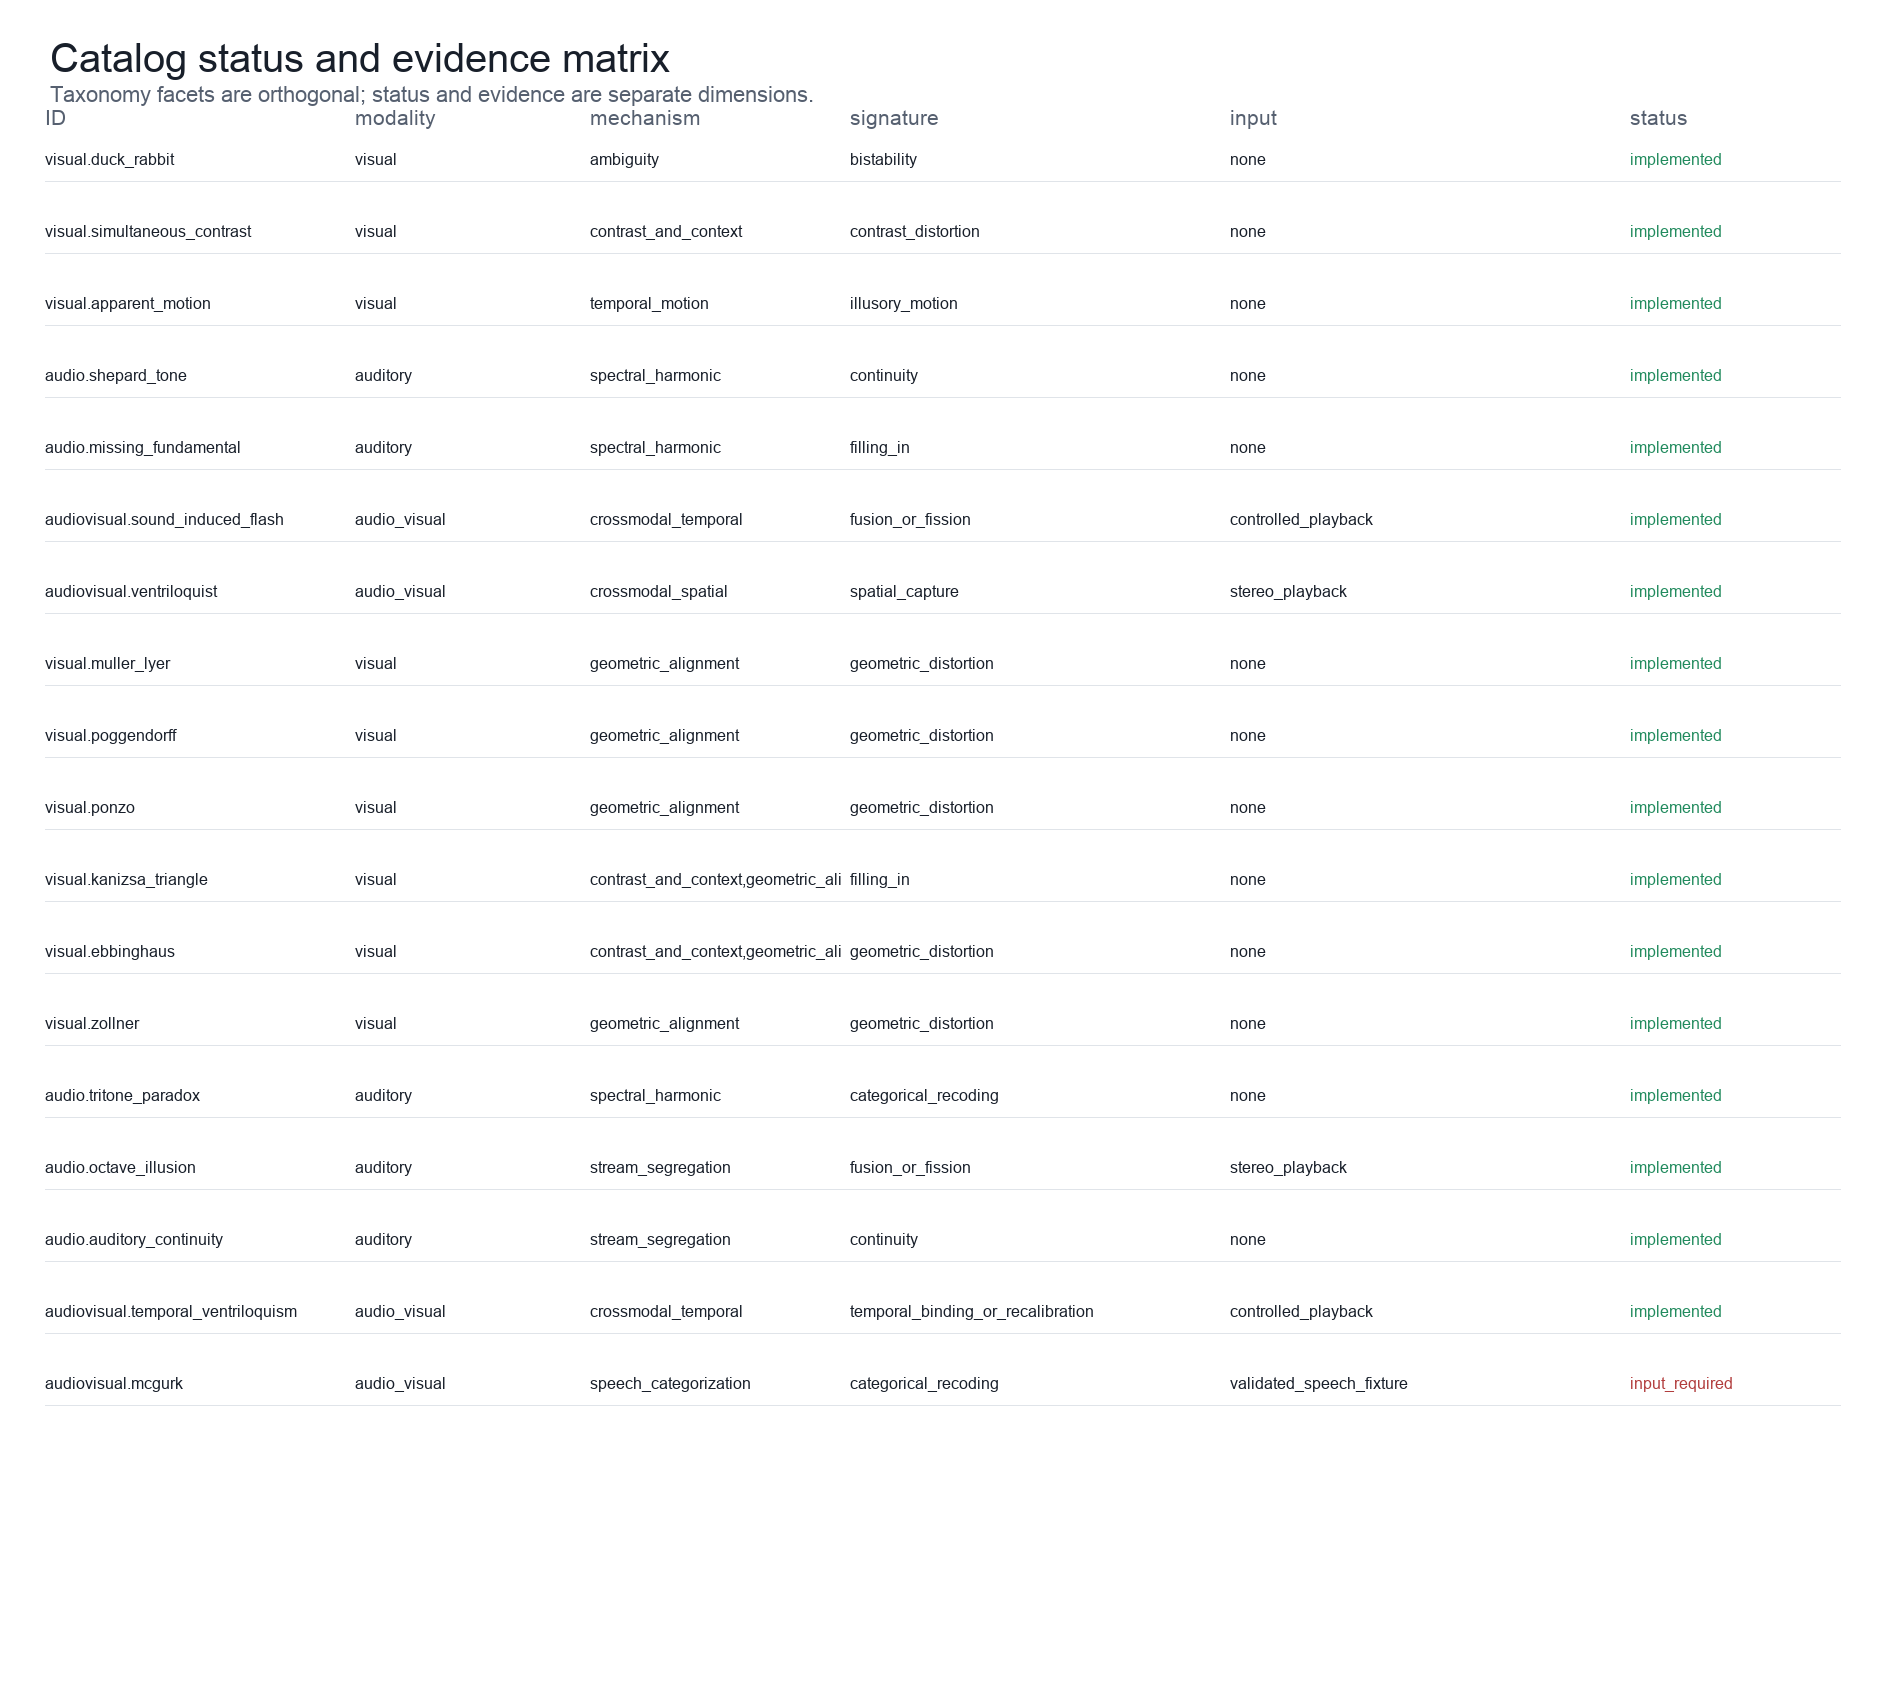
\includegraphics[keepaspectratio,alt={A matrix lists all catalog entries with modality, mechanism, signature, input requirement, and implementation status.}]{../figures/catalog_matrix.png}}
\caption{A matrix lists all catalog entries with modality, mechanism,
signature, input requirement, and implementation
status.}\label{fig:catalog_matrix}
\end{figure}

What this figure shows: A matrix lists all catalog entries with
modality, mechanism, signature, input requirement, and implementation
status. The live catalog matrix contains 18 entries and keeps modality,
mechanism, perceptual signature, input requirement, evidence status, and
implementation status as separate facets. Source data
output/data/catalog\_matrix.json preserve the exact taxonomy snapshot
and its source-reference namespace; status is not a proxy for perceptual
validation. Controls: live taxonomy registry; evidence matrix snapshot;
seed not applicable to the catalog diagram. Objective facts: 18 catalog
rows; categorical facets and statuses; no observer-level quantity is
applicable. Claim level: source\_supported. Source data:
output/data/catalog\_matrix.json (SHA-256 digest recorded in the figure
registry). Evidence lineage: gregory1997visual, hirst2020sound,
bruns2019ventriloquist. Limitations: Taxonomy facets are engineering
classifications and remain provisional where the literature supports
competing accounts. Boundary: Catalog coverage is bounded to this
registered package and does not enumerate all known illusions.

The complete catalog matrix \breakseq{[@fig:catalog\_matrix]} is tabulated in
the standalone Appendix A \breakseq{[@sec:appendix\_catalog; @tbl:catalog]}.
The corresponding machine-readable evidence matrix records the source
role, exact supported claim, engineering departure, and limitation for
every entry. Keeping the table in an appendix gives the main results
narrative room to explain the contract without turning a mutable
registry snapshot into a prose claim.
\end{frame}

\begin{frame}[allowframebreaks]{Typed domains and delivery profiles}
\protect\phantomsection\label{typed-domains-and-delivery-profiles}
\begin{longtable}[]{@{}
  >{\raggedright\arraybackslash}p{(\linewidth - 6\tabcolsep) * \real{0.2500}}
  >{\raggedright\arraybackslash}p{(\linewidth - 6\tabcolsep) * \real{0.2500}}
  >{\raggedright\arraybackslash}p{(\linewidth - 6\tabcolsep) * \real{0.2500}}
  >{\raggedright\arraybackslash}p{(\linewidth - 6\tabcolsep) * \real{0.2500}}@{}}
\caption{Typed parameter domains and
units.}\label{tbl:parameters}\tabularnewline
\toprule\noalign{}
\begin{minipage}[b]{\linewidth}\raggedright
Type
\end{minipage} & \begin{minipage}[b]{\linewidth}\raggedright
Unit
\end{minipage} & \begin{minipage}[b]{\linewidth}\raggedright
Validated domain
\end{minipage} & \begin{minipage}[b]{\linewidth}\raggedright
Role
\end{minipage} \\
\midrule\noalign{}
\endfirsthead
\toprule\noalign{}
\begin{minipage}[b]{\linewidth}\raggedright
Type
\end{minipage} & \begin{minipage}[b]{\linewidth}\raggedright
Unit
\end{minipage} & \begin{minipage}[b]{\linewidth}\raggedright
Validated domain
\end{minipage} & \begin{minipage}[b]{\linewidth}\raggedright
Role
\end{minipage} \\
\midrule\noalign{}
\endhead
PixelDimension & pixels & 8--4096 & image/video width and height \\
GrayscaleLevels & levels & 2--256 & representable grayscale levels \\
QuantizationLevels & levels & 2--256 & output quantization buckets \\
FrequencyHz & Hz & \textgreater{} 0 and finite & oscillator and harmonic
frequencies \\
SampleRate & samples/s & 1,000--384,000 & audio sampling clock \\
FrameRate & frames/s & 1--240 & video presentation clock \\
SyncOffsetMs & ms & −10,000--10,000 & audio relative to video \\
SpatialOffset & normalized & −1--1 & declared crossmodal spatial
discrepancy \\
\bottomrule\noalign{}
\end{longtable}

The parameter contracts are summarized in \breakseq{[@tbl:parameters]}. They
constrain physical construction and serialization; they are not
psychophysical scales.

\begin{longtable}[]{@{}
  >{\raggedright\arraybackslash}p{(\linewidth - 8\tabcolsep) * \real{0.2000}}
  >{\raggedright\arraybackslash}p{(\linewidth - 8\tabcolsep) * \real{0.2000}}
  >{\raggedright\arraybackslash}p{(\linewidth - 8\tabcolsep) * \real{0.2000}}
  >{\raggedright\arraybackslash}p{(\linewidth - 8\tabcolsep) * \real{0.2000}}
  >{\raggedright\arraybackslash}p{(\linewidth - 8\tabcolsep) * \real{0.2000}}@{}}
\caption{Encoding profiles and backend
capabilities.}\label{tbl:encodings}\tabularnewline
\toprule\noalign{}
\begin{minipage}[b]{\linewidth}\raggedright
Format
\end{minipage} & \begin{minipage}[b]{\linewidth}\raggedright
Backend
\end{minipage} & \begin{minipage}[b]{\linewidth}\raggedright
Artifact
\end{minipage} & \begin{minipage}[b]{\linewidth}\raggedright
Profile
\end{minipage} & \begin{minipage}[b]{\linewidth}\raggedright
Status
\end{minipage} \\
\midrule\noalign{}
\endfirsthead
\toprule\noalign{}
\begin{minipage}[b]{\linewidth}\raggedright
Format
\end{minipage} & \begin{minipage}[b]{\linewidth}\raggedright
Backend
\end{minipage} & \begin{minipage}[b]{\linewidth}\raggedright
Artifact
\end{minipage} & \begin{minipage}[b]{\linewidth}\raggedright
Profile
\end{minipage} & \begin{minipage}[b]{\linewidth}\raggedright
Status
\end{minipage} \\
\midrule\noalign{}
\endhead
PNG & Pillow & image & lossless uint8 raster & available \\
WAV & python wave & audio & PCM 8/16/24/32-bit & available \\
GIF & Pillow & video & palette animation with declared duration &
available \\
NPZ & NumPy & canonical artifact & exact little-endian float32 archive &
available \\
MP4 & ffmpeg & video/audiovisual & H.264 or muxed MP4; decode inspected
& available \\
\bottomrule\noalign{}
\end{longtable}

The delivery profiles are summarized in \breakseq{[@tbl:encodings]}. Backend
availability is environment-dependent and is recorded at generation
time.

The catalog distinguishes a physical construction from an observer
claim. For example, the sound-induced-flash generator establishes one
flash and one or two beep events on a shared clock; it does not
establish a reported flash count. Similarly, the temporal-ventriloquism
generator exposes a declared timing offset, while the literature reports
observer-dependent temporal judgments under specific tasks and timing
conditions \breakseq{[@vroomen2004temporal]}.
\end{frame}

\begin{frame}[allowframebreaks]{Pipeline and provenance}
\protect\phantomsection\label{pipeline-and-provenance}
\begin{figure}
\centering
\pandocbounded{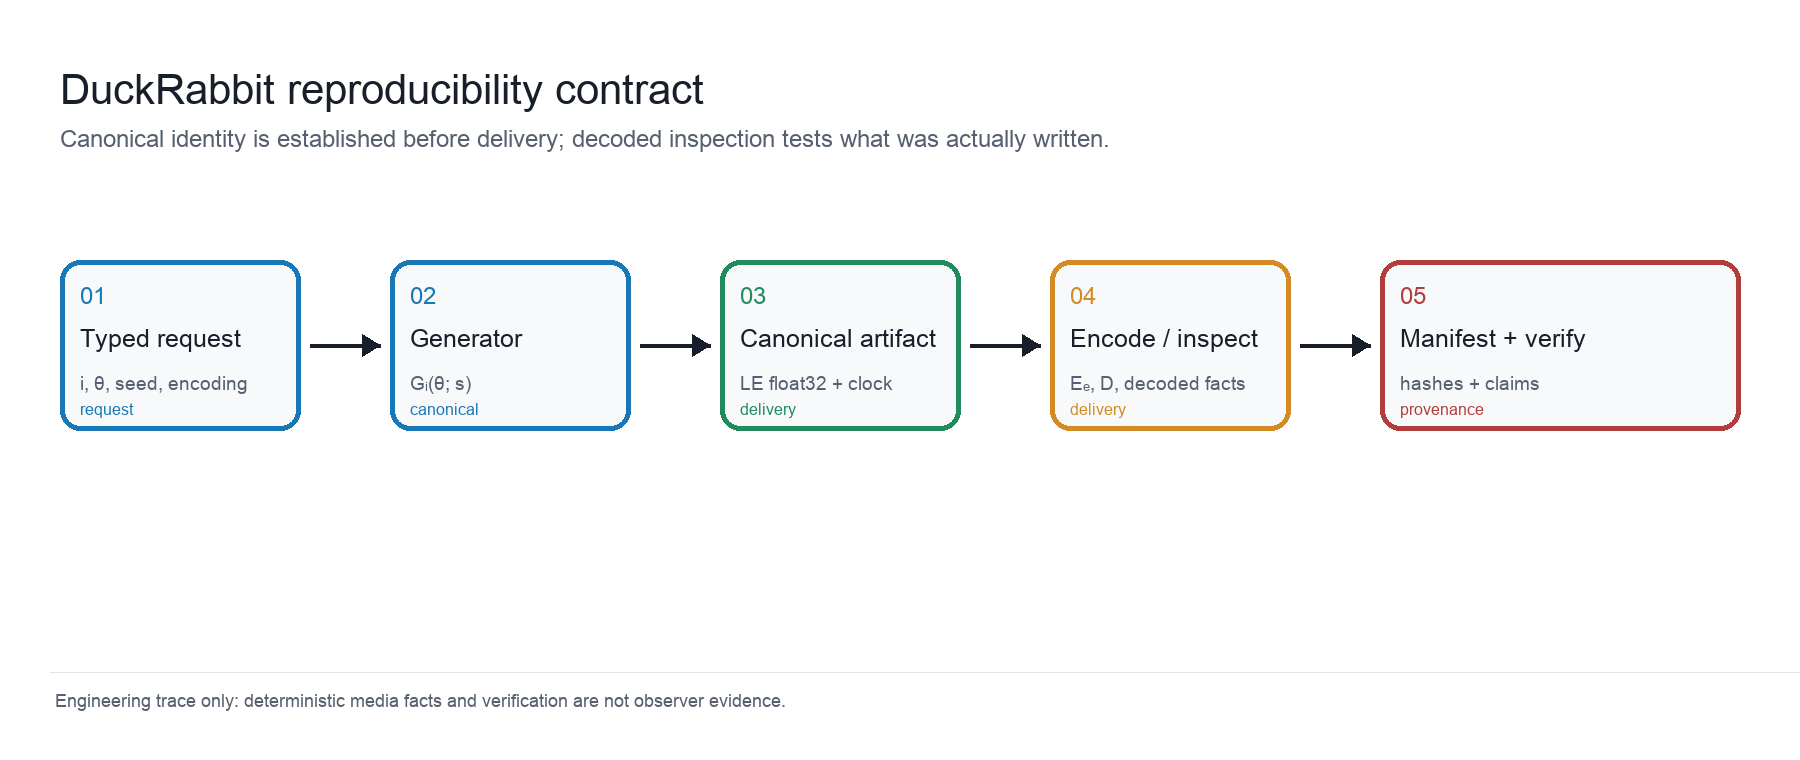
\includegraphics[keepaspectratio,alt={Five labeled stages connect a typed request to a deterministic canonical artifact, encoded media, decoded inspection, and a verification manifest.}]{../figures/architecture.png}}
\caption{Five labeled stages connect a typed request to a deterministic
canonical artifact, encoded media, decoded inspection, and a
verification manifest.}\label{fig:architecture}
\end{figure}

What this figure shows: Five labeled stages connect a typed request to a
deterministic canonical artifact, encoded media, decoded inspection, and
a verification manifest. This schematic separates a typed request from
the canonical artifact it generates, the optional delivery encoder,
decoded inspection, and the manifest-level verification decision. Arrows
indicate data and provenance dependencies rather than a causal model of
perception; the seed is 0 and the complete stage record is in source
data output/data/architecture.json. Controls: typed request q=(i,θ,s,e)
with seed s=0; default generator and delivery-independent
canonicalization. Objective facts: no unit-bearing objective quantity is
applicable to this architecture diagram; stage identities and provenance
fields are recorded in the sidecar. Claim level: canonical\_stimulus.
Source data: output/data/architecture.json (SHA-256 digest recorded in
the figure registry). Evidence lineage: formalism:eq:typed\_request,
formalism:eq:canonical\_generation, formalism:eq:encoding\_verification.
Limitations: The schematic abstracts implementation boundaries and does
not represent an observer study or a causal theory of perception.
Boundary: The pipeline verifies reproducible media facts, not what a
person experiences.

The generated architecture figure \breakseq{[@fig:architecture]} shows the
separation between request, canonical artifact, delivery adapter,
decoded inspection, and manifest. The canonical digest is the identity
of the in-memory stimulus; an encoded hash is the identity of the
delivered file. The difference is intentional.
\end{frame}

\begin{frame}[allowframebreaks]{Visual constructions and parameter
sweeps}
\protect\phantomsection\label{visual-constructions-and-parameter-sweeps}
\begin{figure}
\centering
\pandocbounded{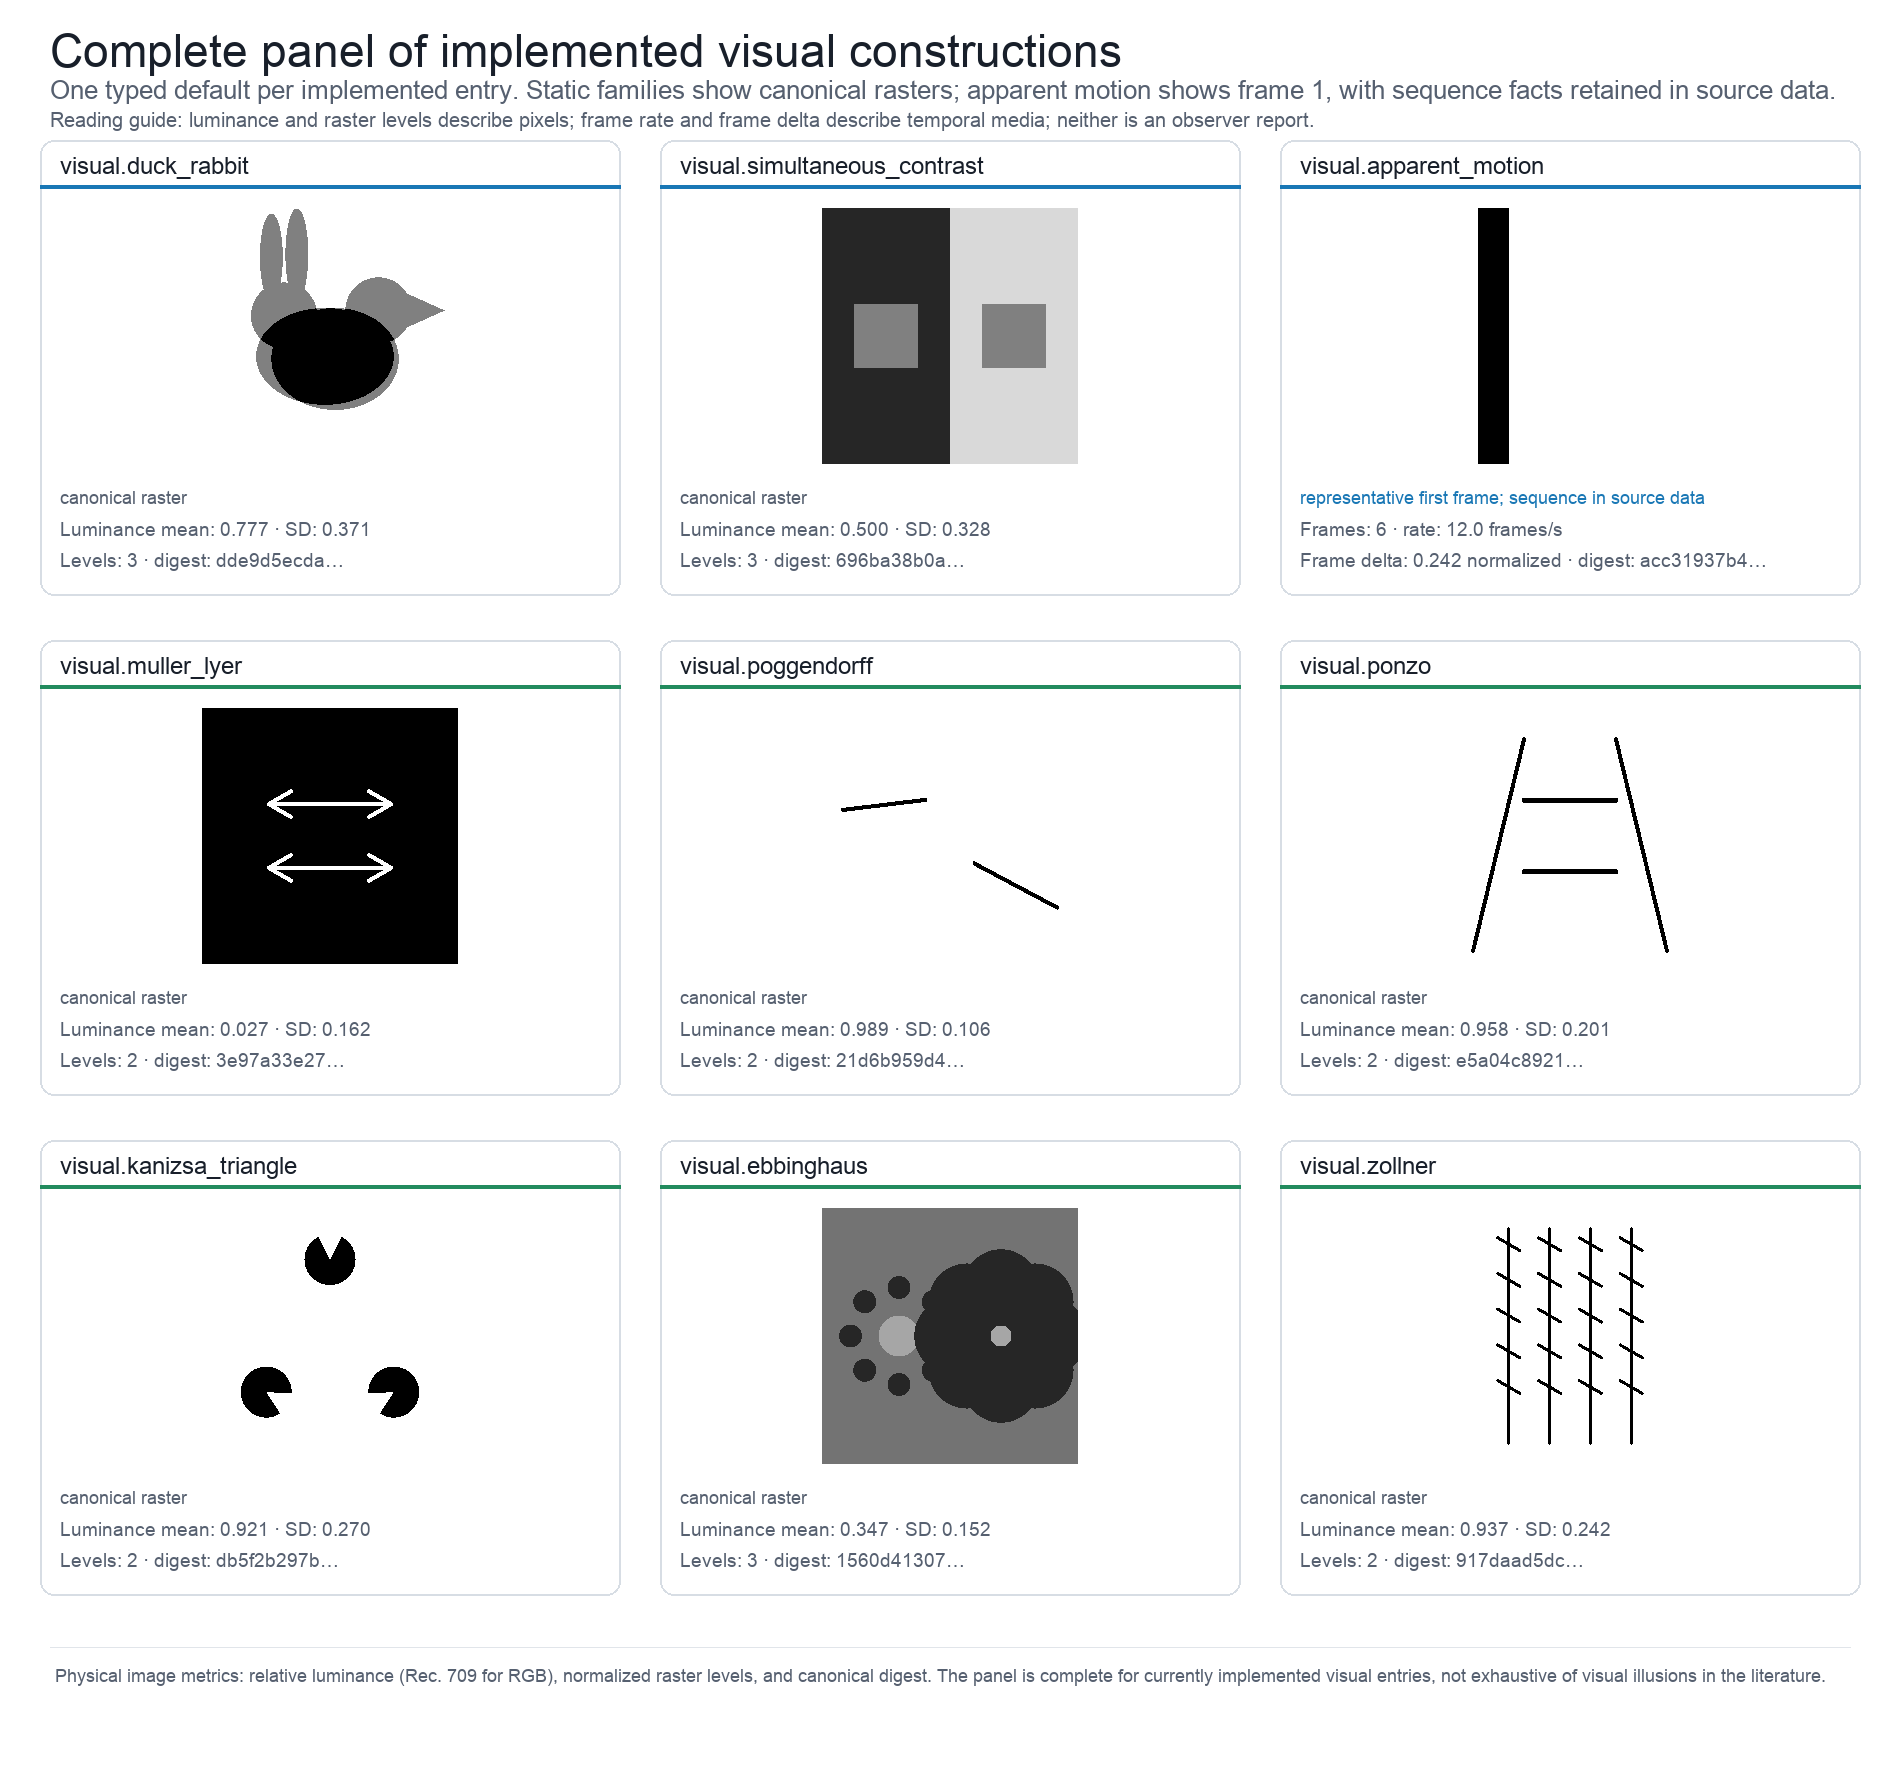
\includegraphics[keepaspectratio,alt={A 9-panel gallery shows every currently implemented visual catalog entry, with stable IDs and physical raster summaries: Duck-rabbit ambiguous figure, Simultaneous contrast stimulus, Apparent-motion frame sequence, Müller-Lyer geometric illusion, Poggendorff geometric illusion, Ponzo perspective illusion, Kanizsa illusory-contour triangle, Ebbinghaus context-size illusion, Zöllner orientation illusion.}]{../figures/visual_panel.png}}
\caption{A 9-panel gallery shows every currently implemented visual
catalog entry, with stable IDs and physical raster summaries:
Duck-rabbit ambiguous figure, Simultaneous contrast stimulus,
Apparent-motion frame sequence, Müller-Lyer geometric illusion,
Poggendorff geometric illusion, Ponzo perspective illusion, Kanizsa
illusory-contour triangle, Ebbinghaus context-size illusion, Zöllner
orientation illusion.}\label{fig:visual_panel}
\end{figure}

What this figure shows: A 9-panel gallery shows every currently
implemented visual catalog entry, with stable IDs and physical raster
summaries: Duck-rabbit ambiguous figure, Simultaneous contrast stimulus,
Apparent-motion frame sequence, Müller-Lyer geometric illusion,
Poggendorff geometric illusion, Ponzo perspective illusion, Kanizsa
illusory-contour triangle, Ebbinghaus context-size illusion, Zöllner
orientation illusion. This complete gallery presents one deterministic
representative from each of the 9 currently implemented visual catalog
entries: Duck-rabbit ambiguous figure, Simultaneous contrast stimulus,
Apparent-motion frame sequence, Müller-Lyer geometric illusion,
Poggendorff geometric illusion, Ponzo perspective illusion, Kanizsa
illusory-contour triangle, Ebbinghaus context-size illusion, Zöllner
orientation illusion. The panel therefore covers the package's available
visual families---ambiguous figure, contrast, apparent motion, geometric
context, illusory contour, contextual size, and orientation-related
constructions---using typed defaults at seed 0. For the temporally
expressed apparent-motion entry, the displayed tile is its first frame
and the source data preserve the full sequence. The source data sidecar
output/data/visual\_panel.json records the stable ID, generator
parameters, canonical SHA-256 digest, Rec. 709 or grayscale luminance
statistics, raster-level counts, and parameter boundary for every tile.
Controls: one default typed parameter object per implemented visual
entry; seed s=0; dimensions, luminance bounds, grayscale, and
quantization controls remain in each generator schema; temporal entries
display their first frame but retain sequence metrics. Objective facts:
per tile: mean and standard-deviation relative luminance, unique raster
levels, and canonical SHA-256 digest; temporal entries additionally
retain frame count, frame rate, and frame deltas; definitions and units
are in the source data JSON. Claim level: canonical\_stimulus. Source
data: output/data/visual\_panel.json (SHA-256 digest recorded in the
figure registry). Evidence lineage: gregory1997visual,
brugger1999duckrabbit, howe2005muller, morgan1999poggendorff,
fisher1967ponzo, yildiz2022ponzo, kanizsa1976contours,
mruczek2015ebbinghaus, earle1995zollner, wertheimer1912motion,
sekuler1996wertheimer. Limitations: The gallery is complete for
implemented visual entries in this package, not a complete survey of
visual illusions; literature families, historical displays, and
DuckRabbit rasters are not pixel-identical by default. Viewing scale,
display calibration, viewing distance, and observer conditions can
change the relevance of a construction; the gallery does not measure an
observer's perceptual report. Boundary: The figure establishes coverage
of the package's implemented visual constructions and their
deterministic raster facts. It does not establish that any viewer will
perceive the named signature, nor that the set is exhaustive of the
visual-illusion literature.

The visual panel \breakseq{[@fig:visual\_panel]} is deliberately a coverage
figure: it contains one deterministic representative for every currently
implemented visual entry, including apparent motion and Zöllner in
addition to the static ambiguous-figure, contrast, geometric-context,
illusory-contour, and contextual- size families. Equalities, masks, line
geometry, luminance bounds, and temporal positions are properties of the
typed rasters or sequences. They are not observer scores, and the
gallery is not an exhaustive ontology of visual illusions.

\begin{figure}
\centering
\pandocbounded{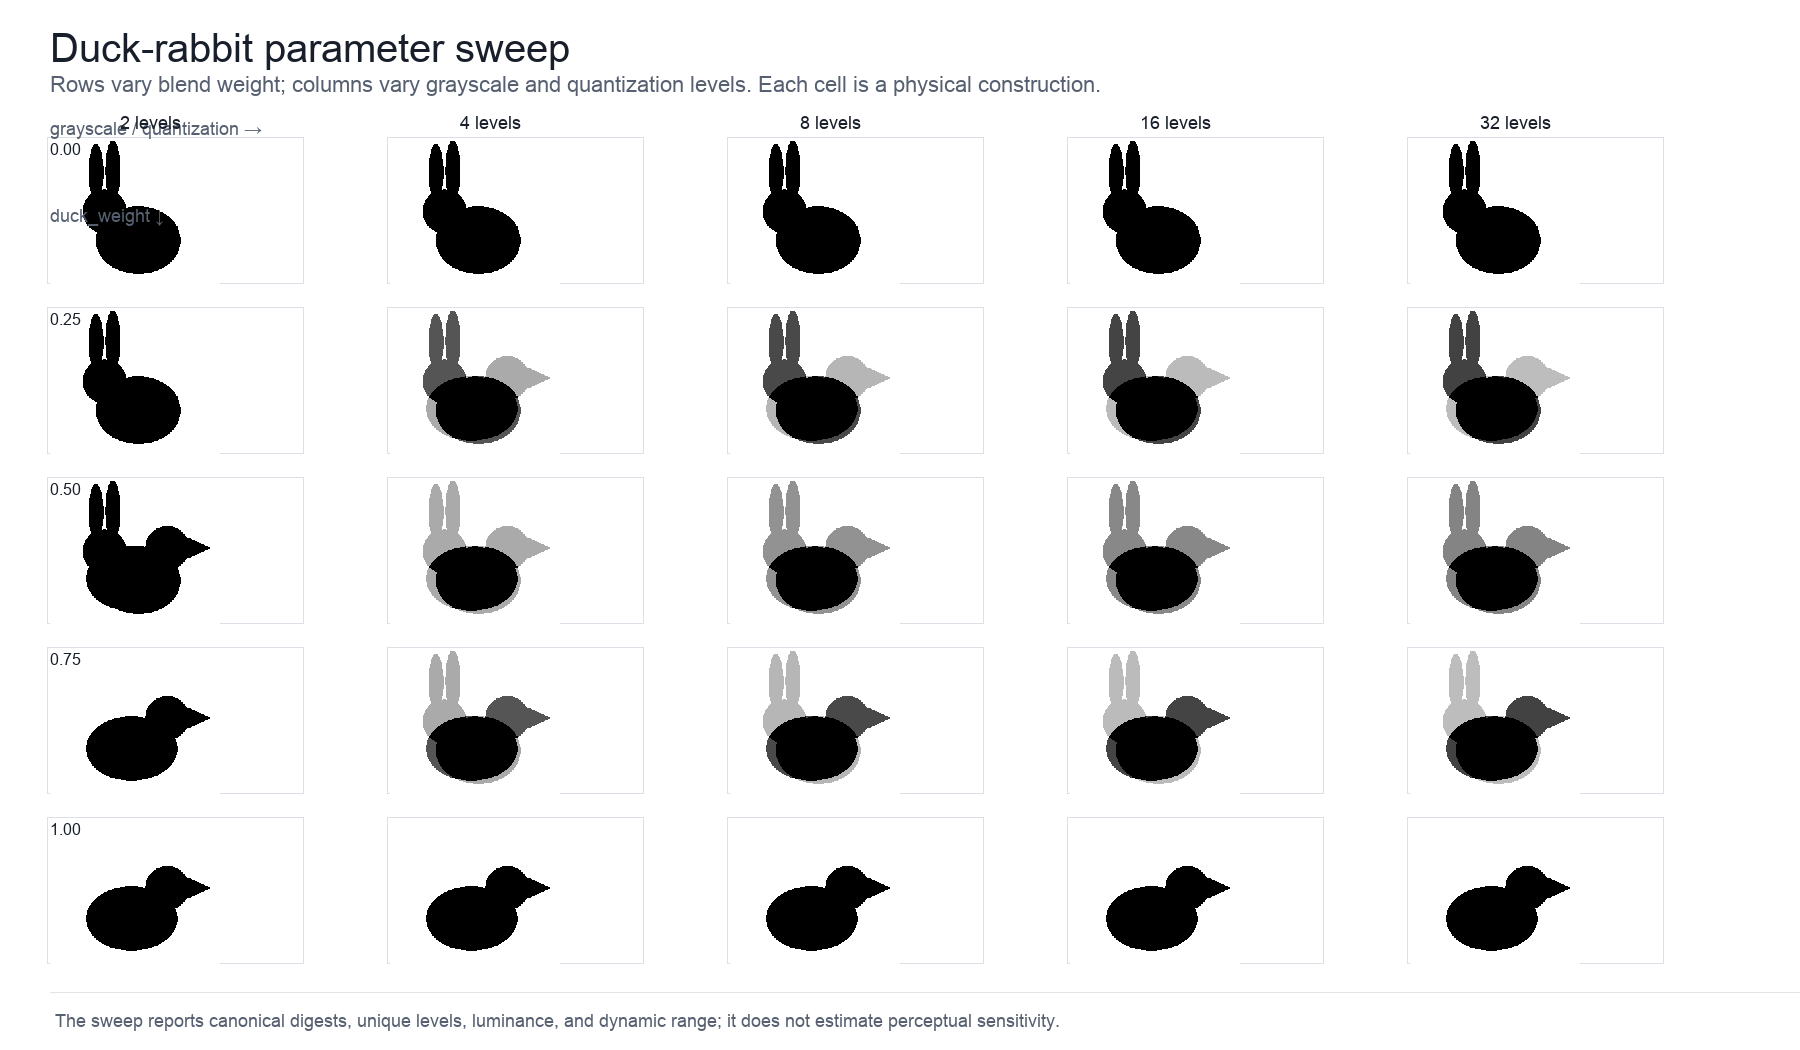
\includegraphics[keepaspectratio,alt={A labeled grid crosses five duck--rabbit blend weights with five grayscale and quantization settings, with physical metrics recorded for each cell.}]{../figures/visual_sweep.png}}
\caption{A labeled grid crosses five duck--rabbit blend weights with
five grayscale and quantization settings, with physical metrics recorded
for each cell.}\label{fig:visual_sweep}
\end{figure}

What this figure shows: A labeled grid crosses five duck--rabbit blend
weights with five grayscale and quantization settings, with physical
metrics recorded for each cell. This 5×5 sweep varies duck--rabbit blend
weight across rows and jointly varies grayscale and quantization levels
across columns. Each cell is regenerated from an immutable typed
parameter object at seed 0; source data output/data/visual\_sweep.json
records canonical digests, unique-level counts, normalized luminance,
and effective dynamic range for every condition. Controls: duck\_weight
∈ \{0,.25,.5,.75,1\}; grayscale=quantization ∈ \{2,4,8,16,32\}; seed
s=0. Objective facts: 25 canonical rasters; unique levels, normalized
mean luminance, and effective dynamic range per cell. Claim level:
physical\_metric. Source data: output/data/visual\_sweep.json (SHA-256
digest recorded in the figure registry). Evidence lineage:
brugger1999duckrabbit, gregory1997visual. Limitations: The grid is a
sensitivity of the construction parameters, not a psychophysical
sensitivity curve or a validated observer effect. Boundary: The chosen
grid is an engineering sampling of the parameter domain and does not
imply an optimal or perceptually uniform spacing.

The sweep \breakseq{[@fig:visual\_sweep]} varies duck-weight from 0 to 1 and
jointly varies representable grayscale and quantization levels. The
source data preserve canonical digests and unique-value counts; no
perceptual score is assigned to a sweep cell.
\end{frame}

\begin{frame}[allowframebreaks]{Temporal and auditory constructions}
\protect\phantomsection\label{temporal-and-auditory-constructions}
\begin{figure}
\centering
\pandocbounded{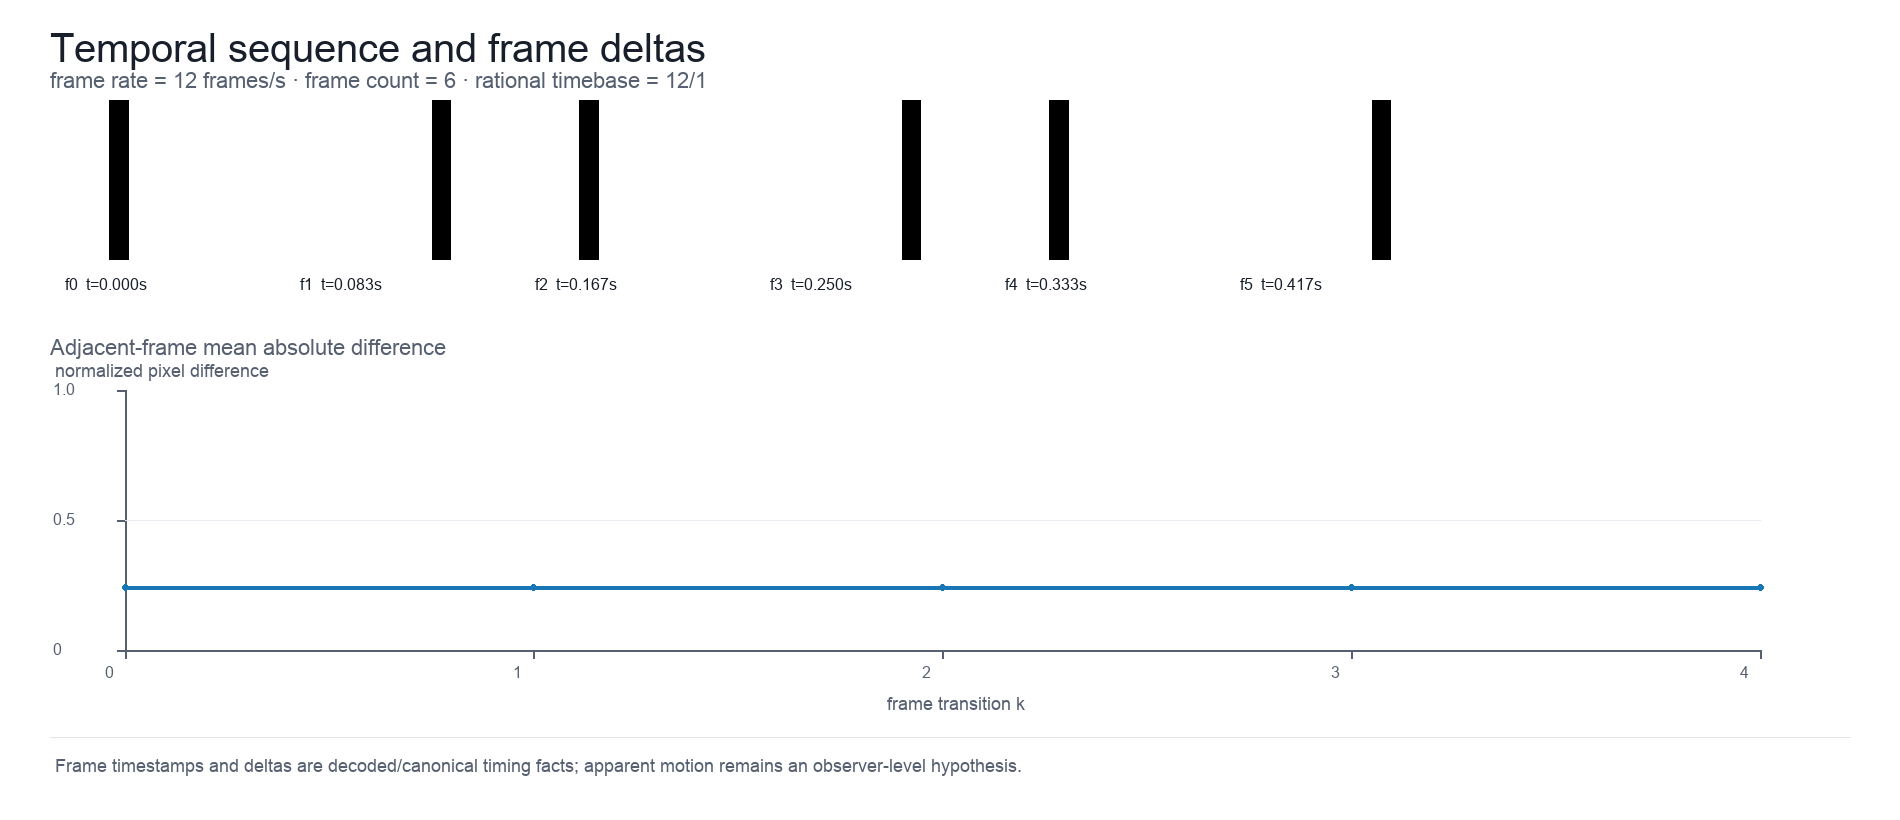
\includegraphics[keepaspectratio,alt={Six ordered frames are labeled with timestamps and paired with a line plot of adjacent-frame normalized pixel differences.}]{../figures/temporal_sequence.png}}
\caption{Six ordered frames are labeled with timestamps and paired with
a line plot of adjacent-frame normalized pixel
differences.}\label{fig:temporal_sequence}
\end{figure}

What this figure shows: Six ordered frames are labeled with timestamps
and paired with a line plot of adjacent-frame normalized pixel
differences. The frame strip exposes the order and timestamps of the
apparent-motion construction, while the lower trace reports
adjacent-frame mean absolute pixel differences. Source data
output/data/temporal\_sequence.json preserve frame count, frame rate,
reduced rational timebase, timestamps in seconds, and the nonzero
transition series; seed 0 identifies the generated sequence. Controls:
visual.apparent\_motion default typed parameters; frame rate and frame
count from the canonical sequence; seed s=0. Objective facts: timestamps
in seconds, frame rate in frames/s, frame count, rational timebase, and
adjacent-frame normalized pixel difference. Claim level:
physical\_metric. Source data: output/data/temporal\_sequence.json
(SHA-256 digest recorded in the figure registry). Evidence lineage:
wertheimer1912motion, sekuler1996wertheimer. Limitations: Frame
succession and frame deltas are physical file properties; playback
timing, display persistence, and motion reports require a controlled
observer task. Boundary: The figure documents temporal structure rather
than the presence, direction, or strength of perceived motion.

The temporal figure \breakseq{[@fig:temporal\_sequence]} reports frame
succession, rational frame rate, and frame-to-frame mean absolute
differences. These facts establish temporal structure in the file, not
the presence or strength of perceived motion.

\begin{figure}
\centering
\pandocbounded{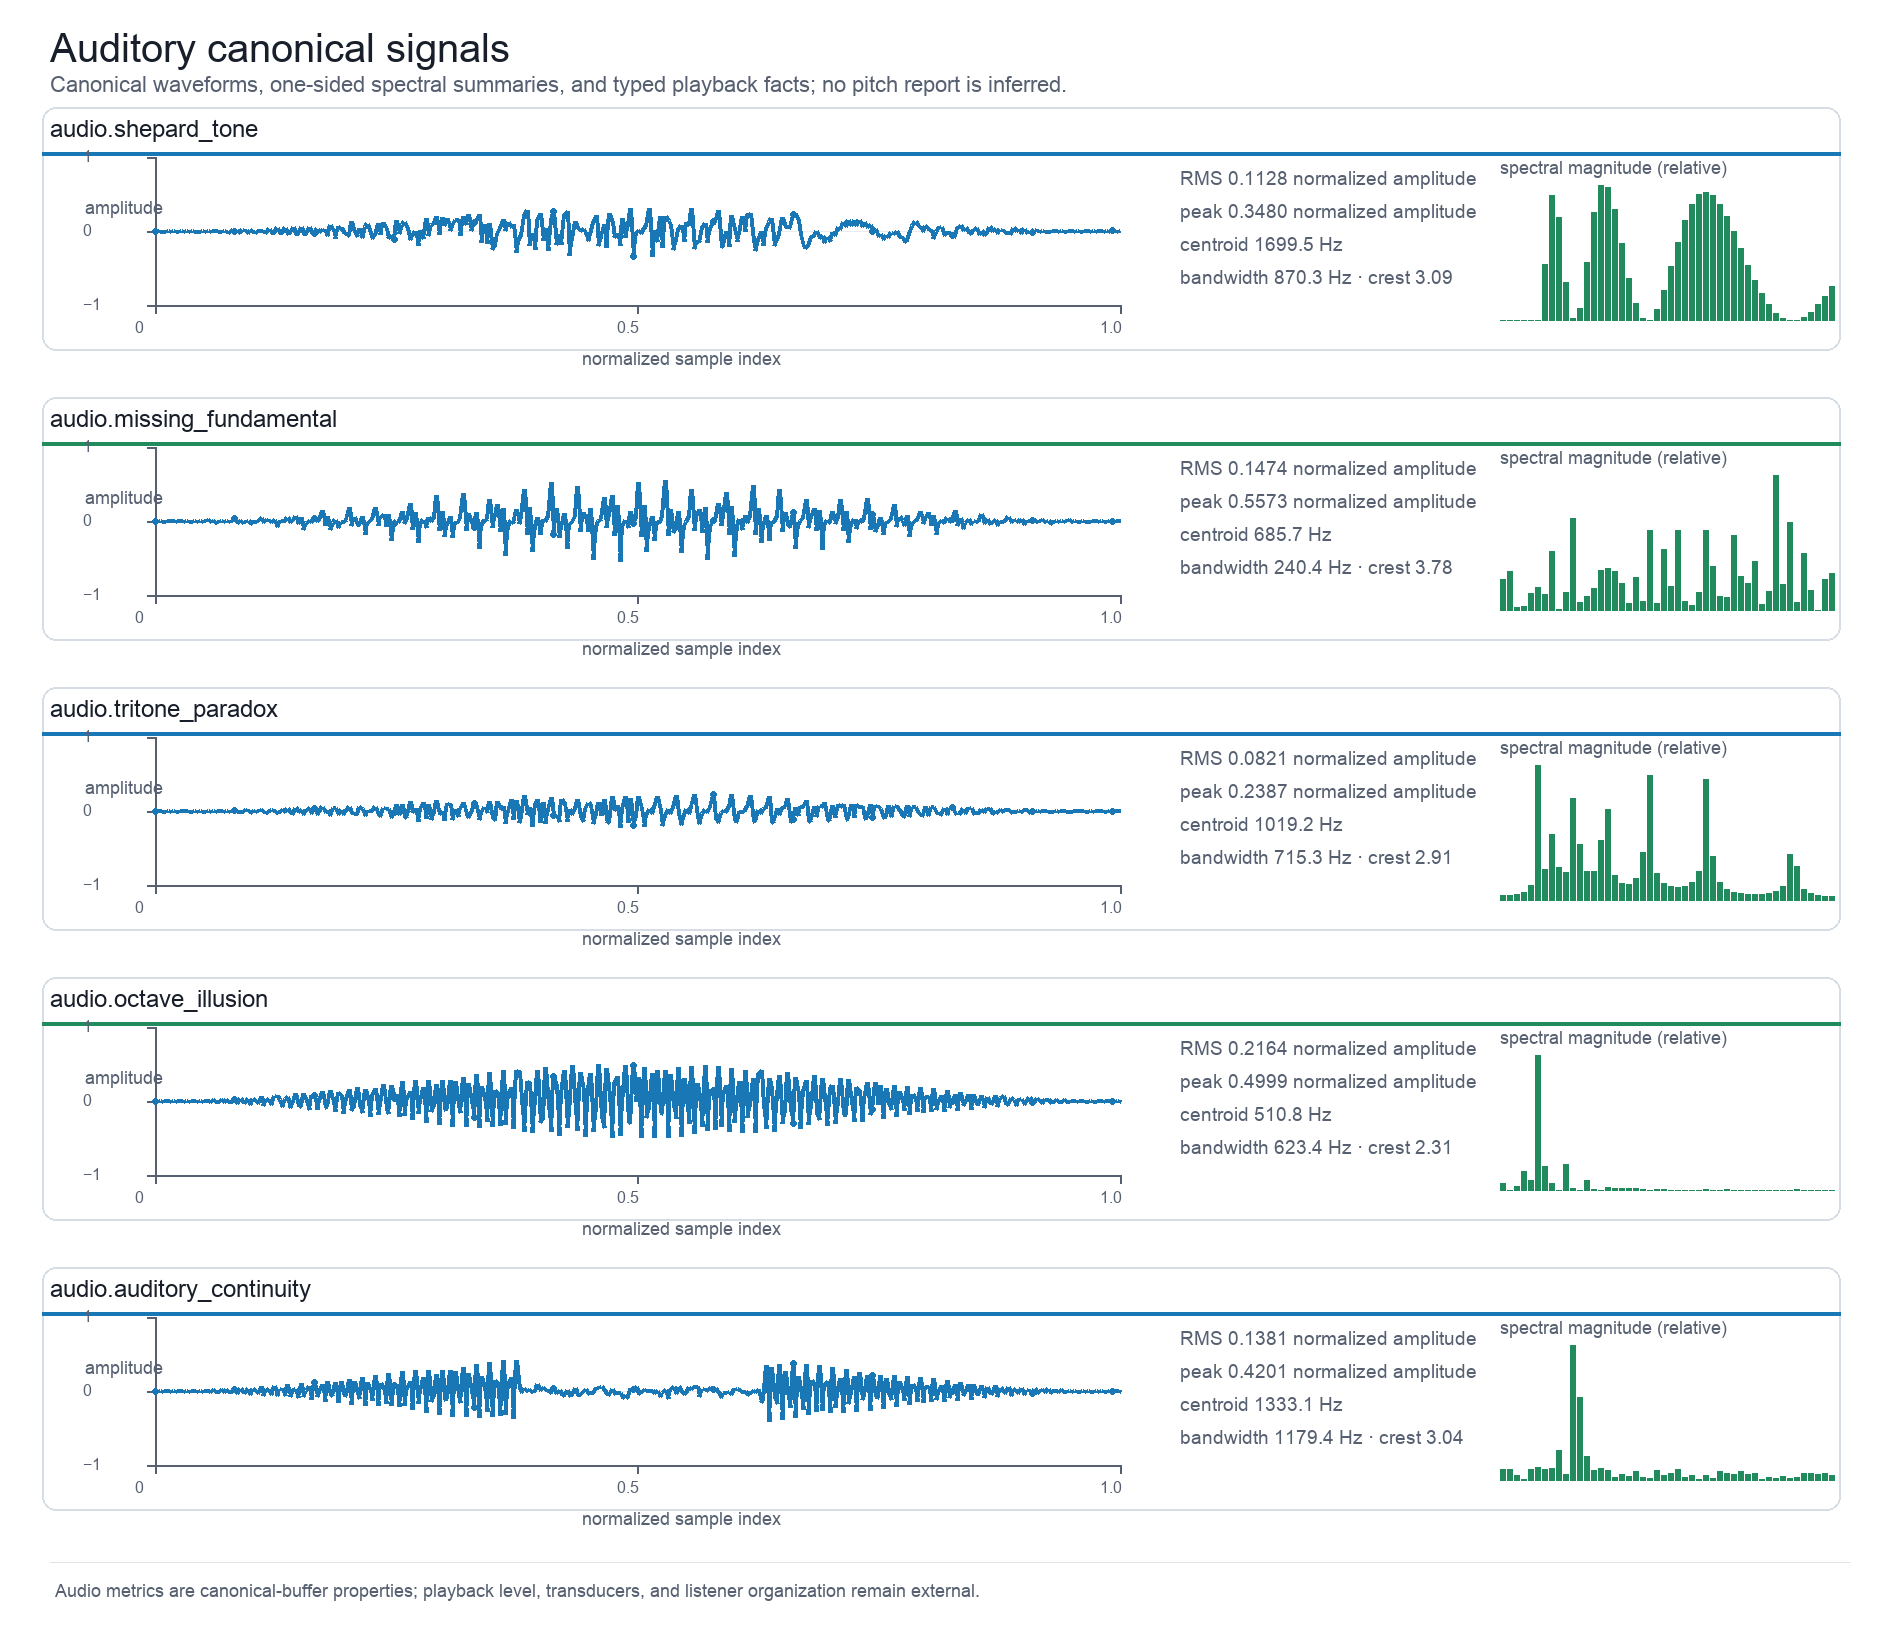
\includegraphics[keepaspectratio,alt={Five labeled rows show canonical audio waveforms, relative one-sided spectral bars, RMS and peak in normalized amplitude, and spectral summaries in hertz.}]{../figures/audio_signals.png}}
\caption{Five labeled rows show canonical audio waveforms, relative
one-sided spectral bars, RMS and peak in normalized amplitude, and
spectral summaries in hertz.}\label{fig:audio_signals}
\end{figure}

What this figure shows: Five labeled rows show canonical audio
waveforms, relative one-sided spectral bars, RMS and peak in normalized
amplitude, and spectral summaries in hertz. Five implemented auditory
constructions---Shepard tone, missing fundamental, tritone paradox,
octave illusion, and auditory continuity---are shown as canonical
waveforms with compact one-sided FFT summaries. Source data
output/data/audio\_signals.json records sample rate, channel layout,
RMS, peak, spectral centroid, bandwidth, crest factor, canonical digest,
and the declared display-bin convention; no pitch or stream report is
inferred. Controls: default typed audio parameters; per-generator
channel layout and sample rate; seed s=0; one-sided FFT display with 48
sampled bins. Objective facts: RMS and peak in normalized amplitude;
spectral centroid and bandwidth in Hz; sample rate in samples/s; channel
layout and canonical SHA-256 digest. Claim level: physical\_metric.
Source data: output/data/audio\_signals.json (SHA-256 digest recorded in
the figure registry). Evidence lineage: shepard1984scale,
zatorre2005missing, deutsch1986tritone, repp1997tritone,
deutsch1974octave, warren1970continuity, riecke2011continuity.
Limitations: Playback level, transducer response, dichotic separation,
masker design, and listener judgments are external to the canonical
buffer. Boundary: The figure compares generated signal properties and
literature-linked families; it does not establish pitch, continuity, or
stream organization for a listener.

The auditory figure \breakseq{[@fig:audio\_signals]} shows canonical waveforms
and spectral summaries for Shepard, missing-fundamental, tritone,
octave, and continuity constructions. RMS, peak, spectral centroid,
bandwidth, and channel layout are calculated from the canonical buffer
with explicit units and windowing rules. Pitch direction, pitch height,
continuity, and stream organization remain observer-level outcomes that
depend on playback and task conditions.
\end{frame}

\begin{frame}[allowframebreaks]{Audiovisual timing and encoding}
\protect\phantomsection\label{audiovisual-timing-and-encoding}
\begin{figure}
\centering
\pandocbounded{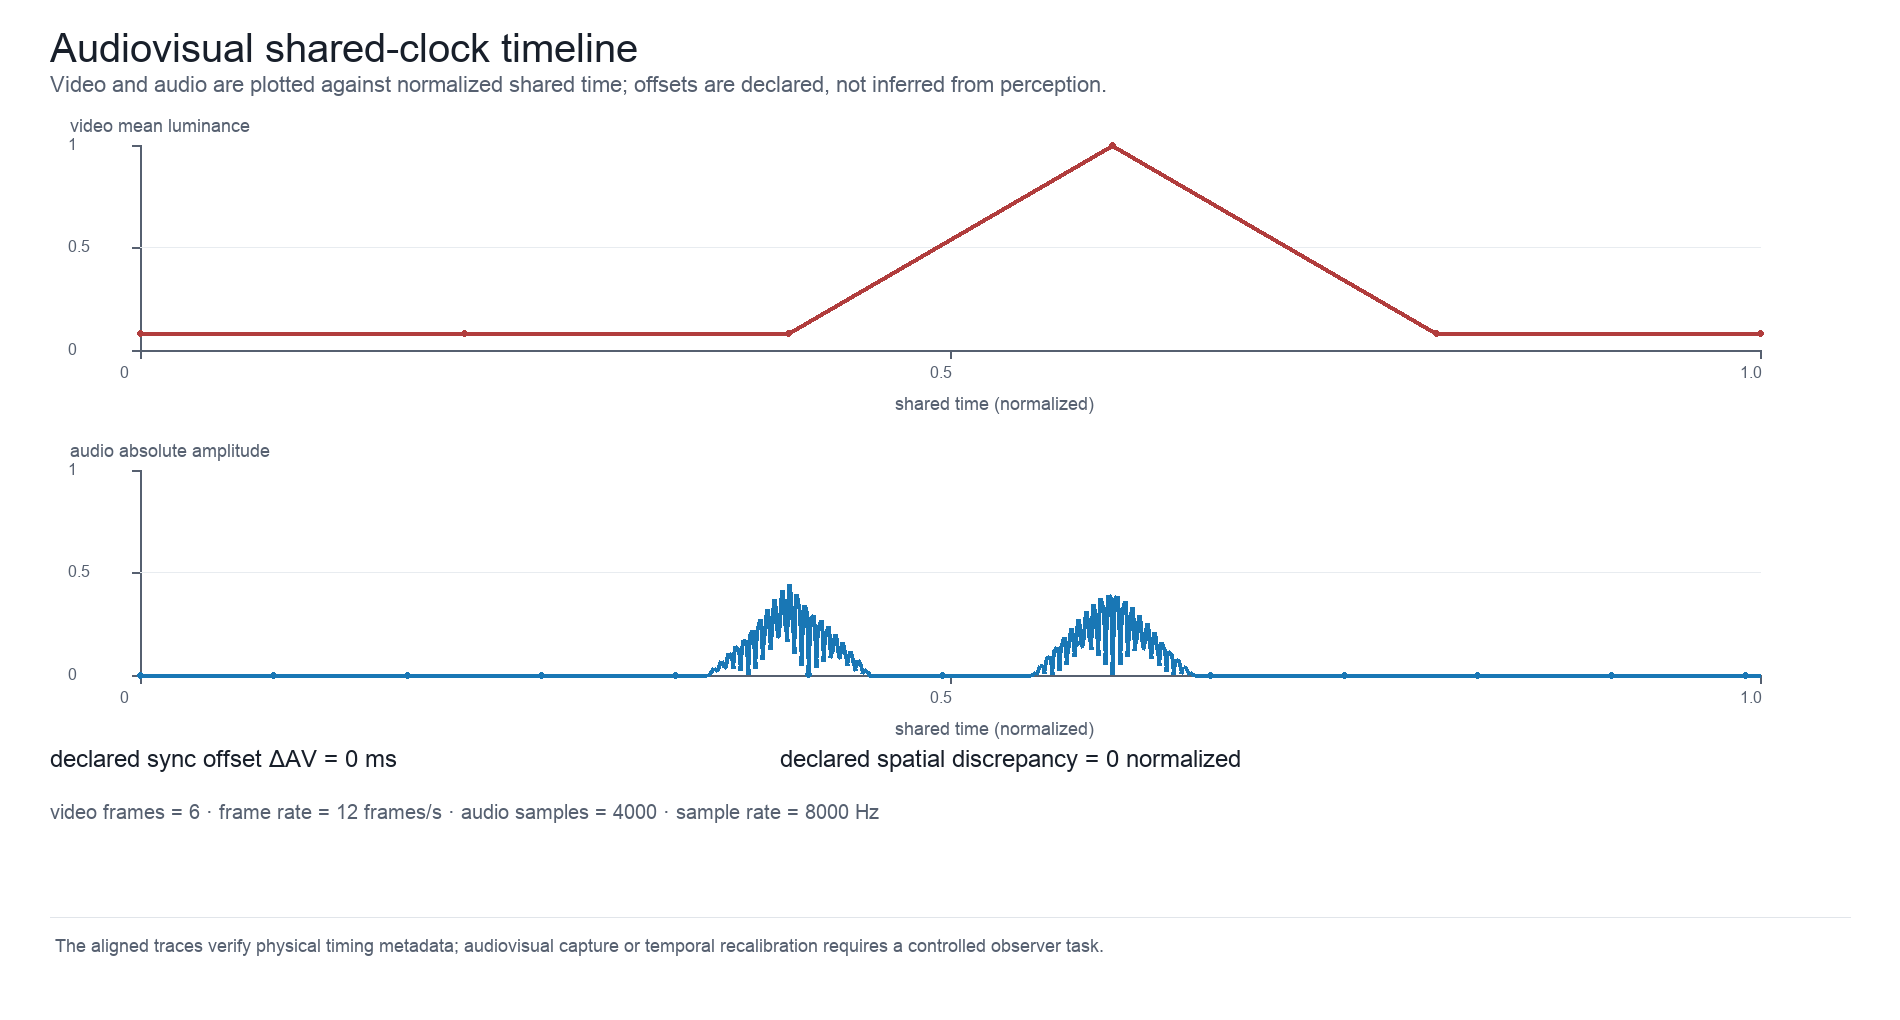
\includegraphics[keepaspectratio,alt={Two labeled traces share a normalized time axis: video mean luminance and audio absolute amplitude, with signed synchronization and spatial offsets printed below.}]{../figures/audiovisual_timeline.png}}
\caption{Two labeled traces share a normalized time axis: video mean
luminance and audio absolute amplitude, with signed synchronization and
spatial offsets printed below.}\label{fig:audiovisual_timeline}
\end{figure}

What this figure shows: Two labeled traces share a normalized time axis:
video mean luminance and audio absolute amplitude, with signed
synchronization and spatial offsets printed below. Video mean luminance
and rectified audio amplitude are placed on a common normalized time
axis for the sound-induced-flash construction. Source data
output/data/audiovisual\_timeline.json records the video frame clock,
audio sampling clock, event traces, signed audio-minus-video
synchronization offset in milliseconds, and normalized spatial
discrepancy; alignment is declared by the generator, not estimated from
perception. Controls: audiovisual.sound\_induced\_flash default shared
timeline; declared sync offset ΔAV and spatial offset; seed s=0.
Objective facts: video luminance and audio envelope on normalized shared
time; ΔAV in ms; spatial discrepancy in normalized units; frame and
sample clocks in the sidecar. Claim level: physical\_metric. Source
data: output/data/audiovisual\_timeline.json (SHA-256 digest recorded in
the figure registry). Evidence lineage: shams2000sifi, hirst2020sound,
vroomen2004temporal, hartcherobrien2011temporal. Limitations: Display
refresh, audio hardware, event latency, and observer temporal binding
are not measured by this figure. Boundary: A shared-clock construction
is not evidence that observers bind the events at the declared or any
other perceptual time.

The audiovisual timeline \breakseq{[@fig:audiovisual\_timeline]} displays video
luminance and audio amplitude against the shared clock, alongside
declared synchronization and spatial offsets. Ventriloquist stimuli
require stereo playback and spatially resolved display; temporal binding
requires controlled timing and an observer task
\breakseq{[@bruns2019ventriloquist; @vroomen2004temporal]}.

\begin{figure}
\centering
\pandocbounded{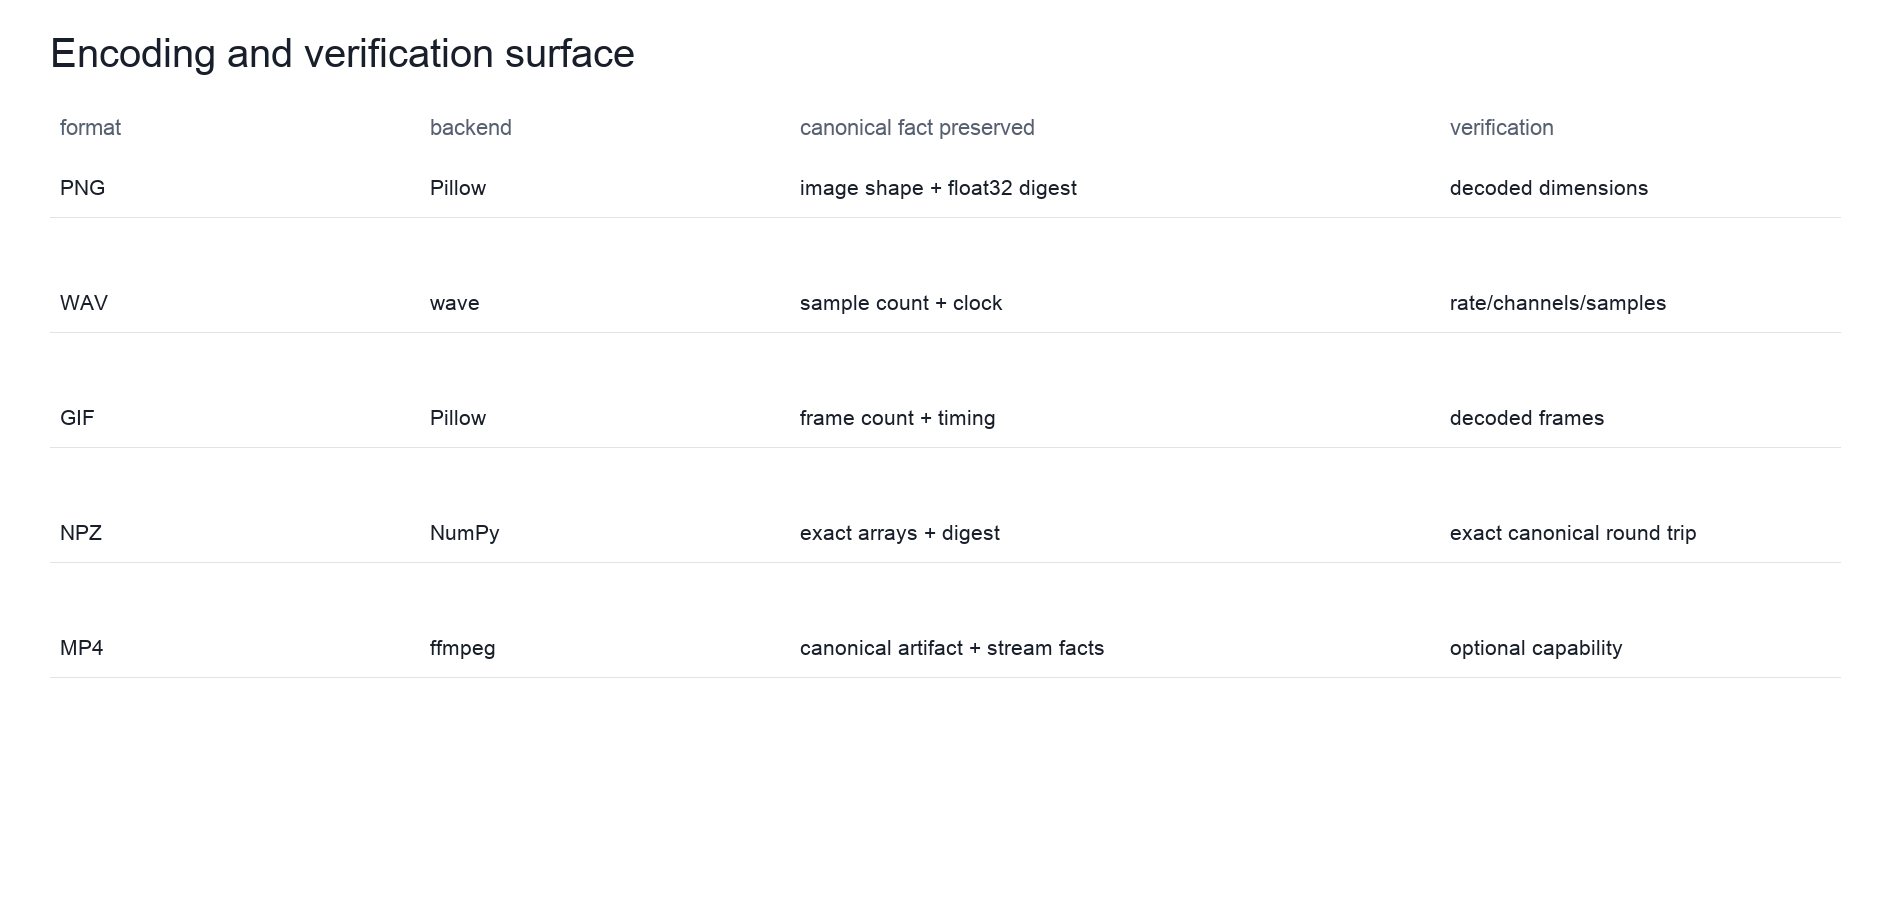
\includegraphics[keepaspectratio,alt={A five-row comparison lists format, backend, preserved canonical facts, and the corresponding decoded verification checks.}]{../figures/encoding_verification.png}}
\caption{A five-row comparison lists format, backend, preserved
canonical facts, and the corresponding decoded verification
checks.}\label{fig:encoding_verification}
\end{figure}

What this figure shows: A five-row comparison lists format, backend,
preserved canonical facts, and the corresponding decoded verification
checks. The comparison separates the canonical artifact from delivery
containers: PNG, WAV, GIF, NPZ, and optional MP4/muxed MP4. Source data
output/data/encoding\_verification.json records backend identity,
preserved canonical facts, decoded inspection targets, and capability
status as observed in the generation environment; the table therefore
describes an adapter contract rather than a claim about codec quality.
Controls: typed encoding profile selected per artifact; overwrite and
backend capability checks; seed inherited from the stimulus request.
Objective facts: format availability and verification scope are
environment observations; NPZ is exact while other formats are decoded
and tolerance-checked. Claim level: encoded\_media. Source data:
output/data/encoding\_verification.json (SHA-256 digest recorded in the
figure registry). Evidence lineage: engineering:typed\_media\_adapters.
Limitations: Backend availability, codec versions, container metadata,
and lossy tolerances are environment-dependent; playback software can
expose additional behavior. Boundary: A successful encode or decode does
not validate an observer effect or guarantee cross-device perceptual
equivalence.

The encoding matrix \breakseq{[@fig:encoding\_verification]} makes backend
capability and verification scope visible. NPZ is the exact canonical
archive; PNG, WAV, GIF, and MP4 are delivery containers whose decoded
facts are checked against the manifest.
\end{frame}

\begin{frame}[allowframebreaks]{Objective metric results}
\protect\phantomsection\label{sec:objective_metric_results}
\begin{longtable}[]{@{}
  >{\raggedright\arraybackslash}p{(\linewidth - 8\tabcolsep) * \real{0.2000}}
  >{\raggedright\arraybackslash}p{(\linewidth - 8\tabcolsep) * \real{0.2000}}
  >{\raggedright\arraybackslash}p{(\linewidth - 8\tabcolsep) * \real{0.2000}}
  >{\raggedright\arraybackslash}p{(\linewidth - 8\tabcolsep) * \real{0.2000}}
  >{\raggedright\arraybackslash}p{(\linewidth - 8\tabcolsep) * \real{0.2000}}@{}}
\caption{Objective metric definitions and epistemic
boundary.}\label{tbl:metrics}\tabularnewline
\toprule\noalign{}
\begin{minipage}[b]{\linewidth}\raggedright
Metric
\end{minipage} & \begin{minipage}[b]{\linewidth}\raggedright
Unit
\end{minipage} & \begin{minipage}[b]{\linewidth}\raggedright
Definition
\end{minipage} & \begin{minipage}[b]{\linewidth}\raggedright
Tolerance
\end{minipage} & \begin{minipage}[b]{\linewidth}\raggedright
Claim level
\end{minipage} \\
\midrule\noalign{}
\endfirsthead
\toprule\noalign{}
\begin{minipage}[b]{\linewidth}\raggedright
Metric
\end{minipage} & \begin{minipage}[b]{\linewidth}\raggedright
Unit
\end{minipage} & \begin{minipage}[b]{\linewidth}\raggedright
Definition
\end{minipage} & \begin{minipage}[b]{\linewidth}\raggedright
Tolerance
\end{minipage} & \begin{minipage}[b]{\linewidth}\raggedright
Claim level
\end{minipage} \\
\midrule\noalign{}
\endhead
mean\_luminance & normalized\_luminance & mean Rec. 709 relative
luminance (grayscale is identity) & exact canonical &
physical\_metric \\
unique\_values & levels & count of distinct canonical image values &
exact integer & physical\_metric \\
rms & normalized\_amplitude & root-mean-square audio amplitude & finite
scalar & physical\_metric \\
peak & normalized\_amplitude & maximum absolute audio amplitude & finite
scalar & physical\_metric \\
spectral\_centroid\_hz & Hz & energy-weighted one-sided spectral
centroid & finite scalar & physical\_metric \\
spectral\_bandwidth\_hz & Hz & spectral standard deviation around the
one-sided centroid & finite scalar & physical\_metric \\
crest\_factor & ratio & audio peak divided by RMS with zero-RMS guard &
finite scalar & physical\_metric \\
mean\_temporal\_delta & normalized\_pixel\_difference & mean
adjacent-frame absolute difference & finite scalar & physical\_metric \\
sync\_offset & ms & declared audio-minus-video offset & typed value &
physical\_metric \\
\bottomrule\noalign{}
\end{longtable}

The metric definitions in \breakseq{[@tbl:metrics]} are computed from canonical
or decoded artifacts and do not encode observer interpretations.

The default duck-rabbit artifact contains 3 unique raster levels and has
mean normalized luminance 0.7770. These values are live generated facts,
not perceptual effect sizes.
\end{frame}

\begin{frame}[allowframebreaks]{Observer estimands and verification
controls}
\protect\phantomsection\label{observer-estimands-and-verification-controls}
\begin{longtable}[]{@{}
  >{\raggedright\arraybackslash}p{(\linewidth - 6\tabcolsep) * \real{0.2500}}
  >{\raggedright\arraybackslash}p{(\linewidth - 6\tabcolsep) * \real{0.2500}}
  >{\raggedright\arraybackslash}p{(\linewidth - 6\tabcolsep) * \real{0.2500}}
  >{\raggedright\arraybackslash}p{(\linewidth - 6\tabcolsep) * \real{0.2500}}@{}}
\caption{Data-free observer outcomes and preregistered
estimands.}\label{tbl:observer_estimands}\tabularnewline
\toprule\noalign{}
\begin{minipage}[b]{\linewidth}\raggedright
Estimand
\end{minipage} & \begin{minipage}[b]{\linewidth}\raggedright
Response and model
\end{minipage} & \begin{minipage}[b]{\linewidth}\raggedright
Reference and contrast
\end{minipage} & \begin{minipage}[b]{\linewidth}\raggedright
Uncertainty
\end{minipage} \\
\midrule\noalign{}
\endfirsthead
\toprule\noalign{}
\begin{minipage}[b]{\linewidth}\raggedright
Estimand
\end{minipage} & \begin{minipage}[b]{\linewidth}\raggedright
Response and model
\end{minipage} & \begin{minipage}[b]{\linewidth}\raggedright
Reference and contrast
\end{minipage} & \begin{minipage}[b]{\linewidth}\raggedright
Uncertainty
\end{minipage} \\
\midrule\noalign{}
\endhead
sifi flash count contrast & event count; poisson or ordinal & sifi one
beep; two-beep minus one-beep event-count response & 95\% confidence
interval \\
temporal binding offset contrast & continuous magnitude; linear mixed &
temporal sync; reported timing shift per declared sync offset & 95\%
confidence interval \\
\bottomrule\noalign{}
\end{longtable}

The analysis contract in \breakseq{[@tbl:observer\_estimands]} specifies
estimands and uncertainty procedures without asserting any result.

\begin{longtable}[]{@{}
  >{\raggedright\arraybackslash}p{(\linewidth - 4\tabcolsep) * \real{0.3333}}
  >{\raggedright\arraybackslash}p{(\linewidth - 4\tabcolsep) * \real{0.3333}}
  >{\raggedright\arraybackslash}p{(\linewidth - 4\tabcolsep) * \real{0.3333}}@{}}
\caption{Verification failure modes and negative
controls.}\label{tbl:verification}\tabularnewline
\toprule\noalign{}
\begin{minipage}[b]{\linewidth}\raggedright
Failure mode
\end{minipage} & \begin{minipage}[b]{\linewidth}\raggedright
Control
\end{minipage} & \begin{minipage}[b]{\linewidth}\raggedright
Expected result
\end{minipage} \\
\midrule\noalign{}
\endfirsthead
\toprule\noalign{}
\begin{minipage}[b]{\linewidth}\raggedright
Failure mode
\end{minipage} & \begin{minipage}[b]{\linewidth}\raggedright
Control
\end{minipage} & \begin{minipage}[b]{\linewidth}\raggedright
Expected result
\end{minipage} \\
\midrule\noalign{}
\endhead
altered encoded file & recompute encoded SHA-256 & fail \\
stale canonical digest & recompute canonical little-endian float32
digest & fail \\
incorrect decoded dimensions & compare inspection facts with manifest
summary & fail \\
stream timing mismatch & compare duration/timebase and declared sync
offset & fail \\
unsupported backend & capability probe before encoding & explicit
capability error \\
conflicting format requests & reject format\_name/output\_spec
disagreement & parameter error \\
\bottomrule\noalign{}
\end{longtable}

The negative controls in \breakseq{[@tbl:verification]} test package integrity
and media contracts; they are not null findings about perception.
\end{frame}

\begin{frame}[fragile,allowframebreaks]{Synthetic psychophysics model
diagnostic}
\protect\phantomsection\label{synthetic-psychophysics-model-diagnostic}
\begin{figure}
\centering
\pandocbounded{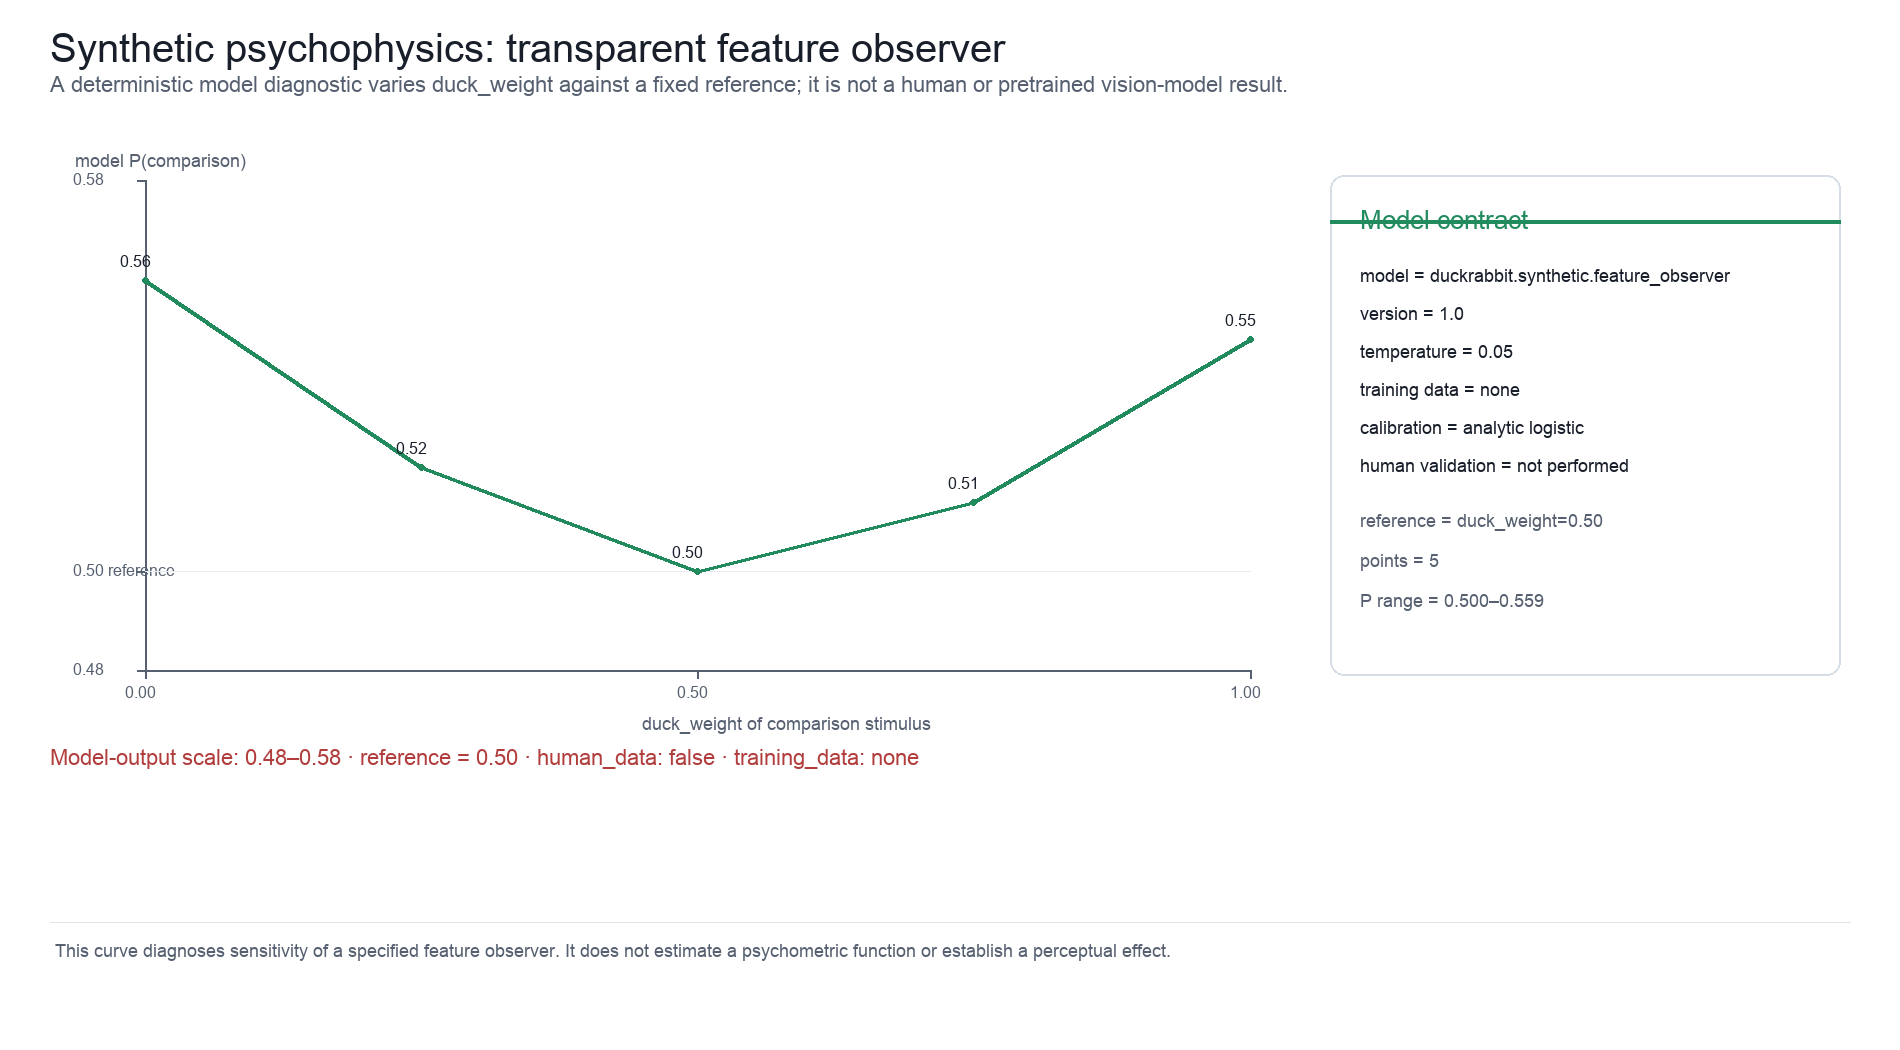
\includegraphics[keepaspectratio,alt={A narrow-range line plot shows deterministic model probability across duck\_weight values beside the model identity, temperature, no-training-data statement, and human-data boundary.}]{../figures/synthetic_psychophysics.png}}
\caption{A narrow-range line plot shows deterministic model probability
across duck\_weight values beside the model identity, temperature,
no-training-data statement, and human-data
boundary.}\label{fig:synthetic_psychophysics}
\end{figure}

What this figure shows: A narrow-range line plot shows deterministic
model probability across duck\_weight values beside the model identity,
temperature, no-training-data statement, and human-data boundary. The
hand-specified feature observer compares duck\_weight variants with a
fixed canonical reference. Its probability trace is computed
analytically from serialized features, weights, and temperature; source
data output/data/synthetic\_psychophysics.json records model ID/version,
reference and comparison digests, seed, calibration,
\breaktt{training\_data=none}, and \breaktt{human\_data=false}. The y-axis
is deliberately a narrow model-output range rather than a human
psychometric scale. Controls: duck\_weight comparison against fixed
reference; serialized feature weights and temperature; seed s=0.
Objective facts: model probability and score delta on the displayed
model-output scale; canonical stimulus digests; human\_data=false;
training\_data=none. Claim level: synthetic\_model\_output. Source data:
output/data/synthetic\_psychophysics.json (SHA-256 digest recorded in
the figure registry). Evidence lineage:
observer:preregistered\_estimands. Limitations: The model is
hand-specified, has no training data, has not been calibrated against
observers, and does not estimate a human threshold or effect size. Its
probabilities are model outputs, not participant responses or a
psychometric function. Boundary: This diagnostic tests deterministic
orchestration and metamorphic input-output behavior only; empirical
psychophysics remains future work.

The diagnostic \breakseq{[@fig:synthetic\_psychophysics]} evaluates a fully
serialized, hand-specified feature observer against a fixed canonical
reference while varying \texttt{duck\_weight}. Its logistic
probabilities are model outputs generated from explicit features,
weights, temperature, and seed; they are not a pretrained vision-model
score, a human psychometric function, an assumed human effect size, or
participant data. A future human study would require a preregistered
task, calibrated display and playback, consented participants, exclusion
and missingness rules, and an analysis contract before any observer
claim could be made.
\end{frame}

\end{document}
